\documentclass[a4paper,
		     11pt,
		     DIV12,
		     DIVcalc,
		     headings=normal,
		     oneside,
		     bibliography=totoc,
		     headsepline=false,
		     headinclude]{scrartcl}

% font
\usepackage[utf8]{inputenc}
\usepackage[T1]{fontenc}
\setkomafont{title}{\normalfont\itshape\huge}
\setkomafont{section}{\normalfont\itshape\Large}
\setkomafont{sectioning}{\normalfont}
\setkomafont{subsection}{\normalfont\itshape\large}
\setkomafont{subsubsection}{\normalfont\itshape}
\setkomafont{paragraph}{\normalfont\itshape}
\setkomafont{pagehead}{\rmfamily\scshape}
%\usepackage[automark,komastyle]{scrpage2}

% german; comment out if not needed
%\usepackage[ngerman]{babel}
%\usepackage[german]{varioref} 
%\usepackage{bibgerm}

% enlarge page size
%\usepackage[automark,komastyle]{scrpage2}
%\pagestyle{useheadings}
%\usepackage[cm,headings]{fullpage}
\usepackage[a4paper,total={150mm,240mm}]{geometry}

% often used packages
\usepackage{amsmath}
\usepackage{amsfonts}
\usepackage{amsthm}
\usepackage{amscd}
\usepackage{grffile}
\usepackage{tikz} 
\usepackage{eurosym} 
\usepackage{graphicx}
\usepackage{psfrag}
\usepackage{listings}
\lstset{language=C++, basicstyle=\ttfamily, 
  keywordstyle=\color{black}\bfseries, tabsize=4, stringstyle=\ttfamily,
  commentstyle=\it, extendedchars=true, escapeinside={/*@}{@*/}}
\usepackage{paralist}
\usepackage{curves}
\usepackage{calc}
\usepackage{picinpar}
\usepackage{enumerate}
\usepackage{algpseudocode}
%\usepackage{algorithmic}
%\usepackage{algorithm}
\usepackage{bm}
\usepackage{multibib}
\usepackage{hyperref}
\usepackage{textcase}
\usepackage{nicefrac}

\title{DUNE PDELab Tutorial 00 \\ Piecewise Linear Finite Elements for the Poisson Equation on Simplices}
\author{\textsc{Peter Bastian}\\
  Universität Heidelberg, \\
  Interdisziplinäres Zentrum für Wissenschaftliches Rechnen\\
  Im Neuenheimer Feld 368, D-69120 Heidelberg\\
  \url{Peter.Bastian@iwr.uni-heidelberg.de}
}
\date{\today}

\begin{document}

\maketitle
\tableofcontents
\clearpage

\section{Introduction}

In this tutorial we solve Poisson's equation with piecewise linear conforming 
finite elements on simplicial elements in one, two and three space dimensions. 
This can be considered as the ``hello world''
example in the numerical solution of partial differential equations which
every software should be able to solve easily (well, there are codes which have
difficulties with triangles). We first provide a short review of the problem and
its finite element solution in order to fix the notation. Then we demonstrate
how this problem is solved using DUNE and PDELab.

\subsection*{Depends On} This tutorial depends on no other tutorials.

\section{Problem Formulation}

\subsection{Strong Formulation}

In this tutorial we consider the {\em Poisson equation}
\begin{subequations}
\begin{align}
-\Delta u & = f \qquad\text{in $\Omega$},\label{eq:1a}\\
u &= g \qquad\text{on $\partial\Omega$},\label{eq:1b}
\end{align}
\end{subequations}
where $\Omega\subset\mathbb{R}^d$ (domains are open and connected sets)
is a given, polyhedral domain (elements with curved
boundaries are possible in DUNE but will not be considered here). 
The problem with homogeneous right hand side $f\equiv 0$ is sometimes called
{\em Laplace equation}. This problem 
is one of the basic equations of mathematical physics which describes gravitational
and electric potential as well as stationary heat or groundwater flow.
Poisson's equation is an instance of an {\em elliptic partial differential equation}.
More about modelling with partial differential equations can be found in \cite{Eriksson,BastianII}.

A function $u\in C^2(\Omega)\cap C^0(\bar\Omega)$ 
(the space of twice continuously differentiable functions in $\Omega$ which are continuous
up to the boundary)
is called a {\em strong solution}
if it satisfies equations \eqref{eq:1a}, \eqref{eq:1b} pointwise. 
Condition \eqref{eq:1b} is called a {\em Dirichlet boundary condition}. Boundary conditions
are necessary to render the solution unique and sometimes one speaks also
of a {\em boundary value problem}.
Formally, one often reduces \eqref{eq:1a}, \eqref{eq:1b}
to a problem with homogeneous Dirichlet boundary conditions $g\equiv 0$ as the
starting point for theoretical considerations. We will deliberately not do this
here as it is also not done in the computer implementation of the method. 

\subsection{Weak Formulation}

Existence, uniqeness and stability of solutions, i.e. well-posedness in the
sense of Hadamard, is easier to prove for so-called weak solutions. As the weak
formulation is also the basis of the finite element method we explain it here.

To start with, suppose $u$ is a strong solution of \eqref{eq:1a}, \eqref{eq:1b} and take 
{\em any } function
$v\in C^1(\Omega)\cap C^0(\bar\Omega)$ with $v=0$ on $\partial\Omega$ then we
have by integration by parts:
\begin{equation*}
\int_\Omega (-\Delta u) v \,dx = 
\int_\Omega \nabla u \cdot \nabla v \,dx= \int_\Omega fv \,dx.
\end{equation*}
Observe that the boundary integral $\int_{\partial\Omega} \nabla u\cdot n v\,dx$ vanishes
due to the fact that $v=0$ on $\partial\Omega$. Loosely speaking $v=0$ is a consequence
of the Dirichlet boundary condition $u=g$ on $\partial\Omega$.

Introducing the abbreviations
\begin{equation}
a(u,v) = \int_\Omega \nabla u \cdot \nabla v \,dx, \qquad l(v) = \int_\Omega fv \,dx
\end{equation}
one can on the other hand ask the question: Is there a class,
more specific a vector space, of functions $V$ with $V_g=\{v\in V : 
\text{$v=g$ on $\partial\Omega$}\}$ and $V_0=\{v\in V : 
\text{$v=0$ on $\partial\Omega$}\}$ such that
the problem
\begin{equation}
u \in V_g :\qquad a(u,v) = l(v) \qquad \forall v\in V_0 \label{eq:weakform}
\end{equation}
has a unique solution. The answer is yes and in particular one can prove the following:
\begin{enumerate}[i)]
\item With $V=H^1(\Omega)$, the Sobolev space of functions with square integrable
weak derivatives, the problem \eqref{eq:weakform} has a unique solution provided
the bilinear form $a : V\times V \to \mathbb{R}$ is continuous and coercive on the 
subspace $V_0\subset V$ and the linear form $l: V \to \mathbb{R}$ is also continuous. 
Coercivity on $V_0$ follows from Friedrich's inequality and for the continuity of the right hand
side functional $f\in L^2(\Omega)$ is a sufficient condition.
\item If in addition $u\in C^2(\Omega)\cap C^0(\bar\Omega)$, then the solution
of \eqref{eq:weakform} and \eqref{eq:1a}, \eqref{eq:1b} coincide.
\end{enumerate}
We call \eqref{eq:weakform} the {\em weak formulation} of \eqref{eq:1a}, \eqref{eq:1b}.
As it has a unique solution under more general conditions than \eqref{eq:1a}, \eqref{eq:1b},
e.g. discontinuous right hand side functions $f$, it can be considered as a generalization
of the problem.

\section{The Finite Element Method}

The (conforming) finite element method, in a nutshell, is based on the weak formulation where
the function space $V$ is replaced by a subspace $V_h\subset V$ 
which is {\em finite dimensional}. Here, the subscript $h$ relates to the dimension of the
function space. One major part of the finite element method is to construct such
so-called {\em finite element spaces}.
Typically, finite element spaces are piecewise polynomial functions.
We consider one particular choice, the space of linear functions on simplicial elements.
There are many text books about the finite element method,
a small selection is
\cite{Eriksson,Ern,Ciarlet,Braess,Brenner,Elman2005,GR,WHElliptisch,RannacherII,BastianII}.

\subsection{Finite Element Mesh}

In order to construct a finite element space a finite element mesh is required.
For simplicity we just consider meshes consisting of $d$-simplices, where a simplex
in $d$ dimensions is the convex hull of $d+1$ points $x_{0},\ldots,x_{d}\in\mathbb{R}^d$
(thus a simplex is, by definition, a closed set of points).

The finite element mesh consists of an ordered set
\begin{equation}
\mathcal{X}_h = \{x_1,\ldots,x_N\}
\end{equation}
of points in $\mathbb{R}^d$ called {\em vertices} and an ordered set 
\begin{equation}
\mathcal{T}_h = \{T_1, \ldots, T_M\}
\end{equation}
of $d$-simplices called {\em elements}.
The elements form a partition of the polygonal domain $\Omega$
\begin{equation}
\bigcup_{T\in \mathcal{T}_h} T = \bar\Omega, \quad 
\forall T, T' \in \mathcal{T}_h, T\neq T' : \mathring{T} \cap \mathring{T}' = \emptyset,
\end{equation}
and where each of the vertices $x_{T,0},\ldots,x_{T,d}$  of a $d$-simplex $T\in\mathcal{T}_h$
coincides with a vertex of the set $\mathcal{X}_h$ (and every $x\in\mathcal{X}_h$ is a vertex
of at least one element).

A simplicial mesh is called {\em conforming} if
the intersection of two different elements, $T\cap T'$, is either
empty or a facet (a simplex of lower dimension, i.e. a vertex, edge, face) of {\em both} elements.

The association of the local numbering of vertices within each element 
and the global numbering of vertices in the vertex set is facilitated
via the {\em local to global map} defined by:
\begin{equation}
\forall T\in\mathcal{T}_h, 0\leq i \leq d: g(T,l) = j \Leftrightarrow x_{T,l} = x_{j} .
\end{equation}
The map $g:\mathcal{T}_h\times\{0,\ldots,d\}\to\mathcal{N}$ 
plays also a very important role in the implementation of the finite element method.
Note also that the symbol $g$ is used for the local to global map and the Dirichlet
boundary conditions but it should always be clear from the context which function is meant.

The {\em index set of the vertices} is denoted by $\mathcal{I}_h=\{1,\ldots,N\}$.
It can be partitioned into indices of interior and boundary vertices:
\begin{equation*}
\mathcal{I}_h = \mathcal{I}_h^{int}\cup\mathcal{I}_h^{\partial\Omega},
\quad \mathcal{I}_h^{int} = \{i\in \mathcal{I}_h\,:\, x_i\in\Omega\},
\quad \mathcal{I}_h^{\partial\Omega} = \{i\in \mathcal{I}_h\,:\, x_i\in\partial\Omega\}.
\end{equation*}

In order to illustrate the notation introduced, 
Figure \ref{fig:femesh} shows an example of a conforming finite element
mesh in two space dimensions with its numbering of vertices and elements,
as well as the local to global map.

Finally, by
\begin{equation}
h = \max_{T\in\mathcal{T}_h} \text{diam}(T)
\end{equation}
we denote the {\em mesh size}.

\begin{figure}
\begin{center}
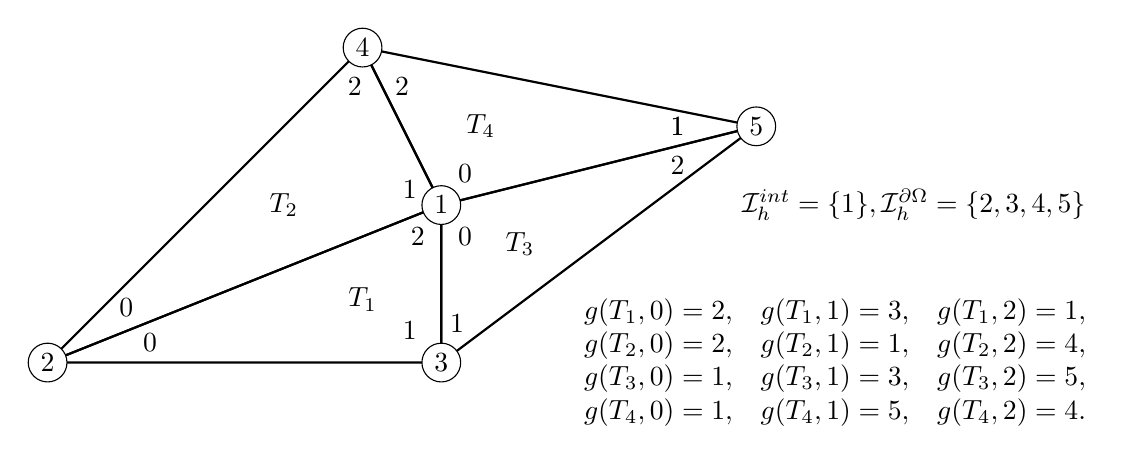
\begin{tikzpicture}[scale=1.0,baseline=(current bounding box.center)]
\draw[thick] (0,0) -- (5,0) -- (5,2) -- cycle;
\draw[thick] (0,0) -- (5,2) -- (4,4) -- cycle;
\draw[thick] (5,0) -- (9,3) -- (5,2) -- cycle;
\draw[thick] (5,2) -- (9,3) -- (4,4) -- cycle;
\node at (4,0.8) {$T_1$};
\node at (3,2) {$T_2$};
\node at (6,1.5) {$T_3$};
\node at (5.5,3) {$T_4$};
\filldraw[fill=white,draw=black] (5,2) circle (7pt) node {$1$};
\filldraw[fill=white,draw=black] (0,0) circle (7pt) node {$2$};
\filldraw[fill=white,draw=black] (5,0) circle (7pt) node {$3$};
\filldraw[fill=white,draw=black] (4,4) circle (7pt) node {$4$};
\filldraw[fill=white,draw=black] (9,3) circle (7pt) node {$5$};
\node at (1.3,0.25) {$0$}; % 2
\node at (1,0.7) {$0$};
\node at (4.6,0.4) {$1$};
\node at (5.2,0.5) {$1$};
\node at (4.7,1.6) {$2$};
\node at (5.3,1.6) {$0$};
\node at (5.3,2.4) {$0$};
\node at (4.6,2.2) {$1$};
\node at (8,2.5) {$2$};
\node at (8,3) {$1$};
\node at (8,3) {$1$};
\node at (3.9,3.5) {$2$};
\node at (4.5,3.5) {$2$};
\node at (10,0) {$%
\begin{array}{lll} 
g(T_1,0) = 2, & g(T_1,1) = 3, & g(T_1,2) = 1, \\
g(T_2,0) = 2, & g(T_2,1) = 1, & g(T_2,2) = 4, \\
g(T_3,0) = 1, & g(T_3,1) = 3, & g(T_3,2) = 5, \\
g(T_4,0) = 1, & g(T_4,1) = 5, & g(T_4,2) = 4.
\end{array}$};
\node at (11,2) {$\mathcal{I}_h^{int}=\{1\}, \mathcal{I}_h^{\partial\Omega}=\{2,3,4,5\}$};
\end{tikzpicture}
\end{center}
\caption{Example of e finite element mesh and the local to global numbering.}
\label{fig:femesh}
\end{figure}

\subsubsection*{Reference Elements and Element Transformation}

The geometry of the mesh elements can be described more easily by
reference elements and an element transformation map. To that end, the
reference $d$-simplex is defined by
\begin{equation*}
\hat T^d = 
\left\{ x\in\mathbb{R}^d \,:\, 0\leq \sum_{i=0}^d (x)_i \leq 1 \wedge \forall i: (x)_i\geq 0 \right \}.
\end{equation*}
The vertices of the reference $d$ simplex are given by
\begin{equation*}
\hat x_0^d = (0,\ldots,0)^T, 
\quad \forall i,j \in \{ 1,\ldots,d\} : (\hat x_i^d)_j = \delta_{i,j}.
\end{equation*}
Figure \ref{fig:refelems} shows the reference elements of dimension 1, 2 and 3
with their numbering of the vertices.

\begin{figure}
\begin{center}
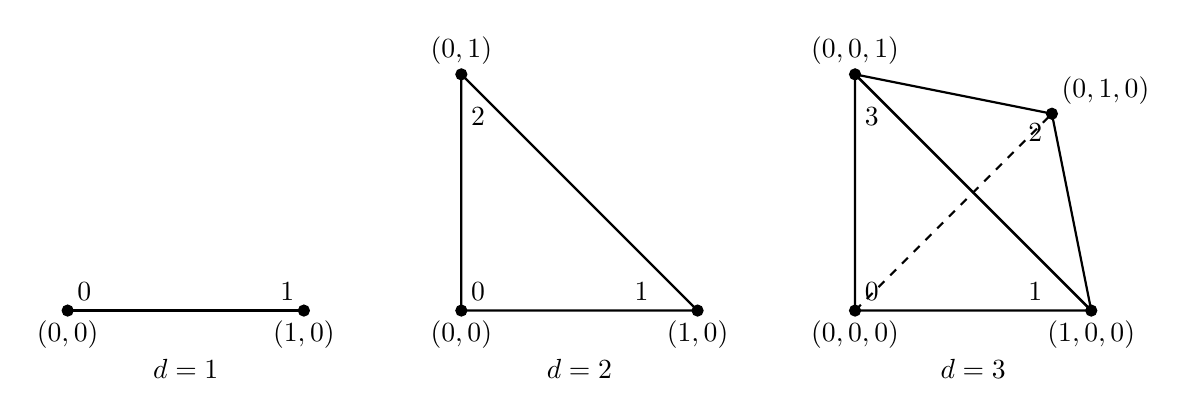
\begin{tikzpicture}[scale=1.0,baseline=(current bounding box.center)]
%d=1
\node[below] at (1.5,-0.5) {$d=1$};
\filldraw (0,0) circle [radius=2pt] node[below] {$(0,0)$}
              (3,0) circle [radius=2pt] node[below] {$(1,0)$};
\draw[thick] (0,0) -- (3,0);
\node[above right] at (0,0) {$0$};
\node[above left] at (3,0) {$1$};
%d=2
\node[below] at (6.5,-0.5) {$d=2$};
\filldraw (5,0) circle [radius=2pt] node[below] {$(0,0)$}
              (8,0) circle [radius=2pt] node[below] {$(1,0)$}
              (5,3) circle [radius=2pt] node[above] {$(0,1)$};
\draw[thick] (5,0) -- (8,0) -- (5,3) -- cycle;
\node[above right] at (5,0) {$0$};
\node[above left] at (7.5,0) {$1$};
\node[below right] at (5,2.7) {$2$};
%d=3
\node[below] at (11.5,-0.5) {$d=3$};
\filldraw (10,0) circle [radius=2pt] node[below] {$(0,0,0)$}
              (13,0) circle [radius=2pt] node[below] {$(1,0,0)$}
              (10,3) circle [radius=2pt] node[above] {$(0,0,1)$}
              (12.5,2.5) circle [radius=2pt] node[above right] {$(0,1,0)$};
\draw[thick] (10,0) -- (13,0) -- (10,3) -- cycle;
\draw[thick] (13,0) -- (12.5,2.5) -- (10,3) -- cycle;
\draw[thick,dashed] (10,0) -- (12.5,2.5);
\node[above right] at (10,0) {$0$};
\node[above left] at (12.5,0) {$1$};
\node[below left] at (12.5,2.5) {$2$};
\node[below right] at (10,2.7) {$3$};
\end{tikzpicture}
\end{center}
\caption{The reference simplices in dimension 1, 2, 3 with vertex positions and
local numbering}
\label{fig:refelems}
\end{figure}

The relation between the reference elements and the elements of the mesh
is provided by the {\em element transformation maps}.
For each element $T\in\mathcal{T}$ there is a map
$$\mu_T : \hat T \to T$$ which maps points of the reference element to the
given element $T$. In an {\em affine} mesh the map $\mu_T$ is affine linear, i.e. it
has the form 
\begin{equation*}
\mu_T(\hat x) = B_T \hat x + a_T
\end{equation*}
for given $d\times d$ matrices $B_T$ and $d$-vectors $a_T$.
Consistency of the local vertex numbering is ensured by the condition
$$\forall i\in\{0,\ldots,d\} : \mu_T(\hat x_i) = x_{T,i}$$.

\subsection{Piecewise Linear Finite Element Functions}

Given a conforming, simplicial and affine finite element mesh in $d$ dimensions we
now can define the space of piecewise linear finite element functions $V_h^1$.
It is given by
\begin{equation}
V_h(\mathcal{T}_h) = \{ v\in C^0(\overline{\Omega}) \,:\, 
\forall T\in\mathcal{T}_h : v|_T\in\mathbb{P}_1^d\}
\label{eq:Vh}
\end{equation}
where $$\mathbb{P}_1^d = \{ p : \mathbb{R}^d \to \mathbb{R}
\,:\, p(x) = a^Tx+ b, a\in\mathbb{R}^d, b\in\mathbb{R}\}$$
is the vector space of multivariate polynomials of degree one in $\mathbb{R}^d$.
It turns out that the condition of continuity is crucial to ensure that $V_h\subset H^1(\Omega)$.
This definition of the finite element space given above does not refer to a basis.
However, for the practical computations one requires a basis for the
finite element space. Analysis reveals that the dimension of the finite element
space $V_h$ is related to the number of vertices of the mesh:
$$\text{dim} V_h = N = \text{dim} \mathcal{X}_h.$$
Therefore, one may construct a basis $\Phi_h=\{\phi_1,\ldots,\phi_N\}$ of $V_h$ 
where each basis function $\phi_i$ is related to vertex $x_i\in\mathcal{X}_h$ in the following way:
\begin{equation*}
\forall i,j\in\mathcal{I}_h \,:\, \phi_i(x_j) = \delta_{i,j}. 
\end{equation*}
A basis with this property is called a {\em Lagrange basis}.
Exploiting this property of the basis we may define the subspace of
finite element functions satisfying homogeneous Dirichlet boundary conditions
\begin{equation*}
V_{h,0} = \{v\in V_h \,:\, \forall i\in\mathcal{I}_h^{\partial\Omega} : v(x_i)=0\}
\end{equation*}
and the set of finite element functions satisfying the
given boundary conditions \eqref{eq:1b}:
\begin{equation*}
V_{h,g} = \{v\in V_h \,:\, \forall i\in\mathcal{I}_h^{\partial\Omega} : v(x_i)=g(x_i)\}.
\end{equation*}
Note that $V_{h,0}$ is a subspace of $V_h$ and satisfies the homogeneous
boundary data exactly whereas $V_{h,g}$ is {\em not} a subspace (it is an affine space)
and only {\em approximates} the given boundary data by piecewise linear functions.
Twodimensional Lagrange basis functions are illustrated in FIgure \ref{fig:p1basis}.

\begin{figure}
\begin{center}
\includegraphics[width=0.4\textwidth]{p1_1}\hspace{0.1\textwidth}
\includegraphics[width=0.4\textwidth]{p1_2}
\end{center}
\caption{Illustration of piecewise linear Lagrange basis functions in 2d. Left one 
corresponds to an interior vertex, right to a boundary vertex.}
\label{fig:p1basis}
\end{figure}

\subsection{Finite Element Solution}

We are now in a position to define and solve the finite element problem.
As pointed out above, the idea is to solve the weak formulation in appropriate
finite-dimensional spaces, i.e.:
\begin{equation*}
u_h\in V_{h,g} : \quad a(u_h,v) = l(v) \quad \forall v\in V_0 .
\label{eq:discrete_weak}
\end{equation*}
Using the Lagrange basis defined above we may expand $u_h\in V_h$ as
\begin{equation*}
u_h = \sum_{j=1}^N (z)_j \phi_j
\end{equation*} 
with coefficient vector $z\in\mathbb{R}^N$. Inserting into the
discrete weak formulation \eqref{eq:discrete_weak} yields:
\begin{align}
a(u_h,v) &= l(v) \quad \forall v\in V_0 &&\text{(discrete weak problem)},\nonumber \\
\Leftrightarrow 
a\left(\sum_{j=1}^N (z)_j \phi_j,\phi_i\right) &= l(\phi_i) \quad \forall i\in \mathcal{I}_h^{int} 
&&\text{(insert basis, linearity)}, \nonumber \\
\Leftrightarrow 
\sum_{j=1}^N (z)_j a\left( \phi_j,\phi_i\right) &= l(\phi_i) \quad \forall i\in \mathcal{I}_h^{int} 
&&\text{(linearity)}. \label{eq:linear1}
\end{align}
The condition $u_h\in V_{h,g}$ can be formulated as a set of equations
\begin{equation}
u_h(x_i) = z_i = g(x_i) \quad\forall i\in\mathcal{I}_h^{\partial\Omega}
\label{eq:linear2}
\end{equation}
which are also linear. Combining the equations \eqref{eq:linear1} and \eqref{eq:linear2}
into a single system of linear equations results in
\begin{equation}
A z = b \label{eq:thesystem}
\end{equation}
where
\begin{equation}
(A)_{i,j} = \left\{\begin{array}{ll}
a(\phi_j,\phi_i) & i\in\mathcal{I}_h^{int}\\
\delta_{i,j} & i\in\mathcal{I}_h^{\partial\Omega}
\end{array}\right., \quad
(b)_{i} = \left\{\begin{array}{ll}
l(\phi_i) & i\in\mathcal{I}_h^{int}\\
g(x_i) & i\in\mathcal{I}_h^{\partial\Omega}
\end{array}\right. .
\label{eq:systemdetail}
\end{equation}
This system may be solved in various ways. The first option are direct solvers
based on some form of the Gaussian elimination technique. However, the matrix $A$
is very sparse as it contains only relatively few nonzero elements per row (3 for $d=1$,
about $7$ for $d=2$ and about $14$ for $d=3$ and Gaussian elimination
may have difficulties to exploit this fact, especially for $d=3$.

Another option is to solve the system iteratively. As the matrix is symmetric and positive
definite there is a variety of methods available which produce, starting from an
initial iterate $z^0$, a convergent sequence $\lim_{k\to\infty} z^k = z$. As a solution
one accepts the first iterate which satisfies the computable criterion
$\|b-Az^k\| < \epsilon \|b-Az^0\|$ for a given reduction factor $\epsilon$.

A very simple (but not very effective) method is {\em Richardson iteration} which is
used to illustrate the concept. It is given by the formula
$$ z^{k+1} = z^{k} + \omega (b-Az^{k}).$$
Algorithmically, this iterative method can be implemented as follows:
\begin{algorithmic}[1]
\State Given $A, b, \epsilon$ and $z$ \Comment{input data}
\State $d = b-Az$ \Comment{compute initial defect}
\State $\tau = \epsilon \|d\|$ \Comment{compute target threshold}
\While{$\|d\|\geq\tau$} \Comment{run until convergence}
\State $z = z + \omega d$ \Comment{update solution}
\State $y = A d$ \Comment{matrix-vector product}
\State $d = d - \omega y$ \Comment{update defect}
\EndWhile
\end{algorithmic}
It can be observed that the matrix $A$ is only involved in matrix-vector
products in lines 2 and 6, an observation that is true for most iterative
solvers. This operation can effectively take into account the sparsity structure
of the matrix and only computations for non-zero elements are necessary.
Thus, one iteration can be implemented with effort $O(N)$. 
The other major factor in the total work is then the number
of iterations needed to achieve the convergence criterion. To keep this
number to an acceptable level effective preconditioners are required.
We do ignore any discussions on effective preconditioners here but they may require 
a major portion of the total work.

Matrix-vector products $y=Az$, require between one and three memory accessess for two
floating point operations as there is never any reuse of the matrix elements.
The exact number depends on the cache reuse of $x$ and $y$ (this is true for
dense and sparse matrices). This fact leads to a very low floating point performance
on modern processors which are much better at computations than at memory access.
A possibility out of this dilemma is to perform the matrix-vector  product in a
{\em matrix-free} fashion, i.e. to recompute the matrix elements while performing
the matrix-vector product instead of storing them. This may lead to a faster 
execution of this operation, especially for certain high-order elements.
Let us consider the matrix-free execution of the matrix-vector product, 
better called {\em operator evaluation}, in more detail.
For $i\in\mathcal{I}_h^{int}$ we get
\begin{equation}
(Az)_i = \sum_{j=1}^N (A)_{i,j} (z)_j = \sum_{j=1}^N a(\phi_j,\phi_i) (z)_j = 
 a\left(\sum_{j=1}^N (z)_j\phi_j,\phi_i\right) = a(u_h,\phi_i) 
\label{eq:opeval}
\end{equation}
where $u_h$ is the finite element function with the coefficients $z$. On the other
hand, for $i\in\mathcal{I}_h^{\partial\Omega}$ we have
\begin{equation*}
(Az)_i = \sum_{j=1}^N \delta_{i,j} (z)_j = (z)_i .
\end{equation*}
We may summarize the typical steps needed to solve the 
finite element problem as follows:
\begin{enumerate}[1)]
\item Assembling the matrix $A$. This mainly involves the computation of the matrix
elements $a(\phi_j,\phi_i)$ and storing them in an appropriate data structure.
\item Assembling the right hand side vector $b$. This mainly involves evaluations of
the right hand side functional $l(\phi_i)$.
\item Perform a matrix free operator evaluation $y=Az$. This involves evaluations
of $a(u_h,\phi_i)$ for all test functions $\phi_i$ and a given function $u_h$.
\end{enumerate}

\subsection{Implementation of the Solution Steps}

We now consider the three operations outlined in the previous section
in more detail. The efficient implementation of these operations involves
the reference elements and the element transformation as part of the following
tools:
\begin{enumerate}[Tool 1)]
\item Transformation formula for integrals. For $T\in\mathcal{T}_h$ we have
\begin{equation*}
\int_T y(x)\,dx = \int_{\hat T} y(\mu_T(\hat x)) \det B_T \,dx .
\end{equation*}
\item Quadrature formula. The midpoint rule reads
\begin{equation*}
\int_{\hat T} q(\hat x) \,dx = q(\hat S_d) w_d
\end{equation*}
where $\hat S_d$ is the center of mass of the reference simplex $\hat T^d$
and $w_d$ is the volume of $\hat T^d$. This quadrature formula is exact for linear
functions.
\item Shape functions. On the reference simplex the linear Lagrange
basis functions are $\hat\phi_i(\hat x) = (\hat x)_i$ for $i>0$ and 
$\hat\phi_0(\hat x) = 1-\sum_{i=1}^d (\hat x)_i$. The basis functions
on a general element $T$ can then be defined via transformation
\begin{equation*}
\phi_{T,i}(\mu_T(\hat x)) = \hat\phi_i(\hat x) .
\end{equation*}
This construction principle can be extend to any function defined on the
reference element. Given $\hat w(\hat x)$ then 
\begin{equation}
w(\mu_T(\hat x))=\hat w(\hat x)
\label{eq:tranformedfunction}
\end{equation}
is the corresponding function on the general element.
\item Computation of gradients. The construction via the reference element
is particularly useful when computing gradients of functions on the general element.
applying the chain rule to \eqref{eq:tranformedfunction} gives
\begin{equation*}
B_T^T \nabla w(\mu_T(\hat x)) = \hat\nabla \hat w(\hat x) \quad\Leftrightarrow\quad
\nabla w(\mu_T(\hat x)) = B_T^{-T}\hat\nabla \hat w(\hat x) .
\end{equation*}
Gradients can be computed by computing gradients on the reference element
and multiplying them with $B_T^{-T}$.
\end{enumerate}
Note that all these tools can be extended to higher order basis functions
and more general element transformations.

\subsubsection*{Assembly of the Right Hand Side}

We start with the assembly of the right hand side vector $b$
defined in equation \eqref{eq:systemdetail}. Since there are typically much more 
interior vertices than boundary vertices we may first compute $(b)_i = l(\phi_i)$
for {\em all} $i\in\mathcal{I}_h$ and then overwrite the entries on the boundary
with $(b)_i = g(x_i)$. Moreover, when considering the global index $i$
only the pairs in the set
$$C(i) = \{(T,m)\in\mathcal{T}_h\times\{0,\ldots,d\} \,:\, g(T,m)=i\}$$
contribute to the computation which can carried out in the following way:
\begin{align*}
(b)_i &= l(\phi_i) = \int_\Omega f \phi_i\,dx &&\text{(definition)} \\
&= \sum_{T\in\mathcal{T}_h} \int_T f \phi_i\,dx &&\text{(use mesh)} \\
&= \sum_{(T,m)\in C(i)} \int_{\hat T} f(\mu_T(\hat x)) \hat\phi_m(\hat x) \det B_T\,dx 
&&\text{(localize)} \\
&= \sum_{(T,m)\in C(i)} 
f(\mu_T(\hat S_d)) \hat\phi_m(\hat S_d) \det B_T w_d \, + \text{error}. &&\text{(employ quadrature)} 
\end{align*}
Note that for general $f$ the integral cannot be computed exactly. The
quadrature formula here only yields exact results for elementwise constant
function $f$ as $\phi_i$ is linear. From now on we ignore this quadrature error

The computations for all components $i\in\mathcal{I}_h$ are now arranged
in such a way that all computations involving element $T$ are carried out together.
These computations at element $T$ are:
\begin{equation*}
(b_T)_m =  f(\mu_T(\hat S_d)) \hat\phi_m(\hat S_d) \det B_T w_d \quad \forall m=0,\ldots,d .
\end{equation*}
Then define the restriction matrix 
$R_T : \mathbb{R}^N \to \mathbb{R}^{d+1}$ as
\begin{equation}
(R_T x)_m = (x)_i \quad \forall \,0\leq m \leq d, \,g(T,m)=i,
\end{equation}
extracting all components involved with element $T$. Then
the assembly of the right hand side can be written in compact form as
\begin{equation}
b = \sum_{T\in\mathcal{T}_h} R_T^T b_T .
\label{eq:rhsassembly}
\end{equation}

\subsubsection*{Assembly of the Matrix}

The assembly of the matrix $A$ defined in \eqref{eq:systemdetail} can be carried
out in a similar way. We assemble first the entries as $(A)_{i,j}=a(\phi_j,\phi_i)$
for all $i,j\in\mathcal{I}_h$ and the modify the matrix to respect the Dirichlet
boundary conditions. In the computation of $(A)_{i,j}$ only the triples
$$C(i,j) = \{(T,m,n)\in\mathcal{T}_h\times\{0,\ldots,d\} \,:\, g(T,m)=i \wedge g(T,n)=j\}$$
are involved due to the locality of the Lagrange basis functions:
\begin{align*}
(A)_{i,j} &= a(\phi_j,\phi_i) = \int_\Omega \nabla \phi_j \cdot \nabla \phi_i \,dx 
&&\text{(definition)}\\
&= \sum_{T\in\mathcal{T}_h} = \int_T \nabla \phi_j \cdot \nabla \phi_i \,dx
&&\text{(use mesh)}\\
&= \sum_{(T,m,n)\in C(i,j)}
\int_{\hat T} (B_T^{-T} \hat\nabla\phi_n(\hat x))\cdot (B_T^{-T} \hat\nabla\phi_m(\hat x))
\det B_T \,d\hat x &&\text{(localize)}\\
&= \sum_{(T,m,n)\in C(i,j)}
(B_T^{-T} \hat\nabla\phi_n(\hat S_d))\cdot (B_T^{-T} \hat\nabla\phi_m(\hat S_d))
\det B_T w_d . &&\text{(quadrature)}
\end{align*}
Note that the quadrature formula is exact since gradients of linear basis functions
and $B_T$ are constant on the element.

Again, the computations are arranged in such a way that all the computations
necessary at a single element are collected. To that end,
the gradients of the basis functions on the reference element (which are {\em independent}
of position) are collected in the $d\times d+1$ matrix
\begin{equation*}
\hat G = \left[\hat\nabla\phi_0(\hat S_d)),\ldots,\hat\nabla\phi_d(\hat S_d))\right] .
\end{equation*}
The matrix $\hat G$ need only be computed once as it does not depend on the
particular element.
With the matrix of transformed gradients $G=B_T^{-T} \hat G$
all computations at element $T$ are 
combined in the so-called {\em local stiffness matrix} given by
\begin{equation*}
A_T = G^T G \det B_T w_d .
\end{equation*}
and the system matrix $A$ can be computed as
\begin{equation}
A =  \sum_{T\in\mathcal{T}_h} R_T^T A_T R_T .
\label{eq:matrixassembly}
\end{equation}

\subsubsection*{Matrix-free Operator Evaluation}

Finally, the considerations above can be applied to the matrix-free operator
evaluation \eqref{eq:opeval}:
\begin{align*}
(Az)_i  &= a(u_h,\phi_i) =  \int_\Omega \nabla u_h \cdot \nabla \phi_i \,dx =
&&\text{(definition)} \\ 
&= \sum_{T\in\mathcal{T}_h} \int_T \nabla u_h \cdot \nabla \phi_i \,dx
&&\text{(use mesh)}\\
&= \sum_{(T,m)\in C(i)}
\int_{\hat T} 
\left(\sum_{n=0}^d (z)_{g(T,n)} B_T^{-T} \hat\nabla\phi_n\right)
\cdot (B_T^{-T} \hat\nabla\phi_m) \det B_T \,d\hat x &&\text{(localize)}\\
&= \sum_{(T,m)\in C(i)}
\left(\sum_{n=0}^d (z)_{g(T,n)} B_T^{-T} \hat\nabla\phi_n\right)
\cdot (B_T^{-T} \hat\nabla\phi_m) \det B_T w_d . &&\text{(quadrature)}
\end{align*}
Again, computations for all indices can be arranged in an element-wise fashion
which reads now
\begin{equation}
Az =  \sum_{T\in\mathcal{T}_h} R_T^T G^T G R_T z.
\label{eq:matrixfreeeval}
\end{equation}

\subsubsection*{Generic Assembly Procedure}

Comparing the formulas \eqref{eq:rhsassembly}, \eqref{eq:matrixassembly}
and \eqref{eq:matrixfreeeval} for the three basic operations necessary for
finite element computations reveals a joint algorithmic form:
\begin{algorithmic}[1]
\For{$T\in\mathcal{T}_h$} \Comment{loop over mesh elements}
\State $z_T = R_T z$ \Comment{load element data}
\State $q_T=\text{compute}(T,z_T)$ \Comment{element local computations}
\State $\text{Accumulate}(q_T)$ \Comment{store result in global data structure}
\EndFor
\end{algorithmic}

It turns out that this basic structure is the same for a huge number
of  finite element and finite volume methods independently of
the partial differential equation to be solved including linear
and nonlinear equations, stationary and time-dependent equations
and even systems of equations. Only the element-local
computations in step (3) need to be exchanged. Therefore PDELab
provides a generic assembler class carrying out steps (1), (2) and (4)
while the element-local computations are supplied by a parameter class.

\section{Realization in PDELab}

\section{Excercises}

% bibtex bibliography
\bibliographystyle{plain}
\bibliography{tutorial00.bib}

\end{document}
